%
% ORIXES DA M�SICA: PATRIMONIO PRIMIXENIO
% ---------------------------------------
%\subsection{O patrimonio musical primixenio} \label{sub:patrimonio}

Dentro das fontes organol�xicas que forman parte do patrimonio musical primixenio, atopamos unha serie de instrumentos musicais moi rudimentarios, recuperados en diferentes escavaci�ns arqueol�xicas. A dificultade de co�ecer realmente a organolox�a empregada na prehistoria � debida � utilizaci�n de materiais perecedoiros na construcci�n dos instrumentos musicais, que presentan maior degradaci�n co paso do tempo.

A percusi�n corporal, percutores de pau, pedras de entrechoque, ax�uxeres (pedras, madeiras, l�minas de metal, area, \ldots); raspadores, aer�fonos feitos de canas de �sos; tambores a partires de troncos de �rbores; trompas feitas de cornos de animais e arpas feitas de arcos de frecha, entre moitos outros, forman parte do gran cat�logo de instrumentos primixenios da prehistoria.


\begin{figure}[h!]
\centering
\subfigure[Arco primitivo]{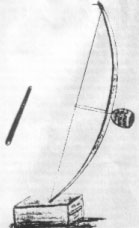
\includegraphics[width=0.25\textwidth]{../figures/ud-00/arco-arpa.jpg}}
\subfigure[Reconstruci�n dunha arpa primitiva]{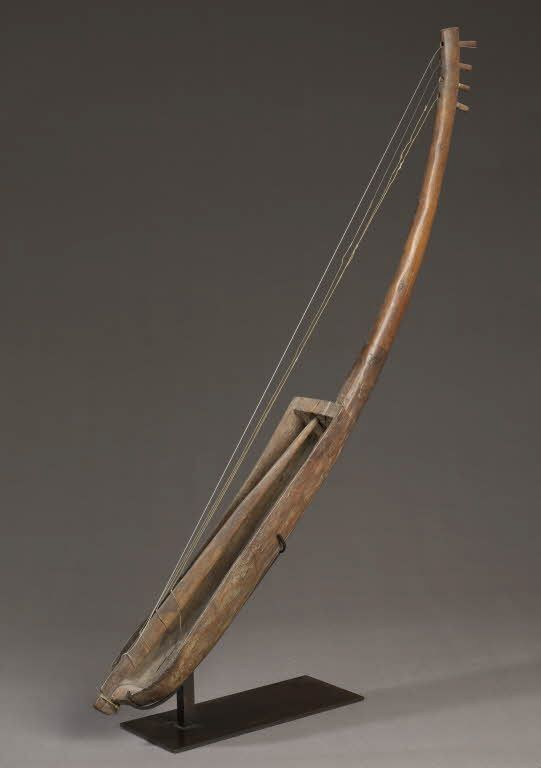
\includegraphics[width=0.29\textwidth]{../figures/ud-00/harpa-louvre.jpg}}
\subfigure[Frauta de �so]{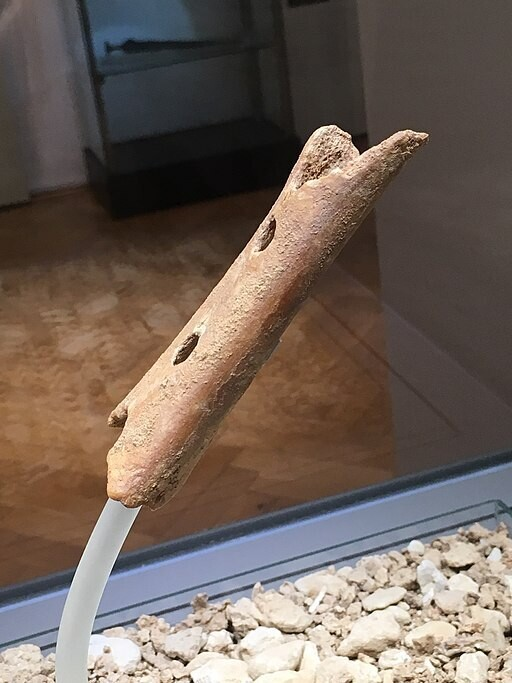
\includegraphics[width=0.31\textwidth]{../figures/ud-00/frauta-oso-museo.jpg}}
\subfigure[Arco africano]{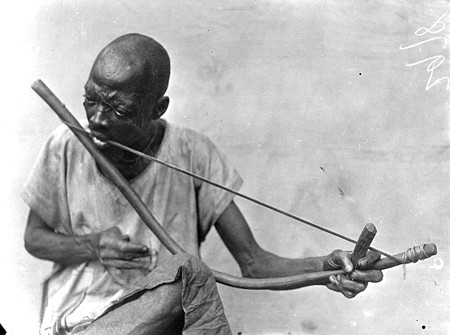
\includegraphics[width=0.50\textwidth]{../figures/ud-00/arco-primitivo.jpg}}
\subfigure[Membran�fono primitivo]{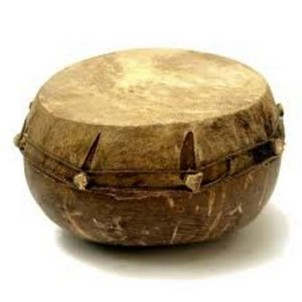
\includegraphics[width=0.35\textwidth]{../figures/ud-00/tambor-primitivo.jpeg}}
\caption{Exemplo de intrumentos que forman parte do patrimonio primixenio musical}
\label{fig:instrumentos-prehistoricos}
\end{figure}


Pouco podemos dicir en cambio, das fontes musicais. Probablemente empregasen escalas de dous a sete sons. En canto �s melod�as, sabemos que eran curtas e sen complexidades; m�is ben sinxelas, empregando intervalos b�sicos de cuartas, quintas e oitavas. Do estudo etnol�xico comparado de tribos da actualidade, deducimos que � probable que empregasen alg�n tipo de polifon�a simple con bord�n
%\sidenote{O \textbf{bord�n} consiste nunha nota mantida, soando � vez que a melod�a.}
ou heterofon�a
%\sidenote{A \textbf{heterofon�a}, neste caso fai referencia a d�as li�as mel�dicas con pequenas variantes.}
.

%Alg�ns exemplos organol�xicos deste patrimonio, podemos observalos na ilustraci�n \ref{fig:instrumentos-prehistoricos}.

